\documentclass[a4paper, 12pt]{article}

\usepackage[portuges]{babel}
\usepackage[utf8]{inputenc}
\usepackage{amsmath}
\usepackage{float}
\usepackage{indentfirst}
\usepackage{graphicx}
\usepackage[colorinlistoftodos]{todonotes}



%\date{\today}

\begin{document}
%\maketitle

\begin{titlepage}
	\begin{center}
		\huge{Universidade Federal de Santa Catarina}

\vspace{10pt}
\begin{figure}[!ht]
\centering
\hspace{0cm}

\includegraphics[height=4cm, width=4cm]{ufsc-logo-2.png}
\end{figure}
        
        \vspace{85pt}
        
		\textbf{\LARGE{Trabalho - Macromodelo de Amplificador de Tensão}}
		\large{\\
        		   }
		\vspace{160pt}
		
	\end{center}
		
	\begin{flushleft}
		\begin{tabbing}
			Aluno\qquad\qquad\= Matheus Francisco Batista Machado\\
			Professor\> Thiago Weber \\
		
	\end{tabbing}
		  
	\end{flushleft}
	
	\begin{center}
		\vspace{\fill}
		Santa Catarina, 02 de março de 2018
	\end{center}
\end{titlepage}
%%%%%%%%%%%%%%%%%%%%%%%%%%%%%%%%%%%%%%%%%%%%%%%%%%%%%%%%%%%
\newpage
\tableofcontents
\thispagestyle{empty}

\newpage
\pagenumbering{arabic}

%%%%%%%%%%%%%%%%%%%%%%%%%%%%%%%%%%%%%%%%%%%%%%%%%%%%%%%%%
%%%%%%%%%%%%%%%%%%%%%%%%%%%%%%%%%%%%%%%%%%%%%%%%%%%%

\section{Equipamentos Utilizados}
Foi utilizado o apenas o software LTSPICE para realizar simulações

\section{Procedimentos}
\subsection{ Macromodelo amplificador}
Considere a Figura 1 onde tem-se um sensor com 1 mV de tensão de entrada e uma resistência em série de 10$\Omega$  
\begin{figure}[H]
\centering
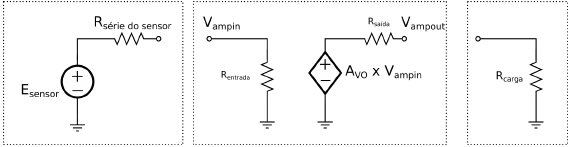
\includegraphics[scale=0.5]{modelo.png}
\caption{Macromodelo amplificador}
\label{Rotulo}
\end{figure}

Busca-se amplificar a tensão de 1 mV para  1V, assim podemos calcular o ganho do amplificador pela fórmula $A_v = \frac{V_{vout}}{V_{in}}$ então tem-se um ganho de  $A_v =\frac{1V}{1mV} = 1000 $.
Utilizando as fórmulas.
\begin{eqnarray*}
V_{in} = V_{s}\frac{R_{in}}{R_{in}+R_{s}}\newline
\\
V_{out}= A_{vo}Vin\frac{R_{carga}}{R_{carga}+R_{out}}\newline
\\
\frac{V_{out}}{V_s} = A_{vo}\frac{R_{in}}{R_{in}+R_{s}}\frac{R_{carga}}{R_{carga}+R_{out}}
\end{eqnarray*}
A figura abaixo mostra o circuito modelado no ltspice
\begin{figure}[H]
\centering
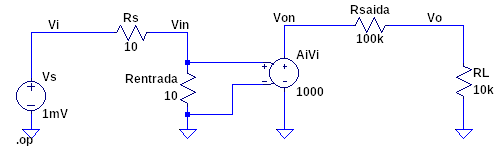
\includegraphics[scale=0.5]{ltspice.png}
\caption{Circuito modelado no ltspice}
\label{Rotulo}
\end{figure}

Na tabela 1 tem-se os ganhos calculados e simulados para os casos de resistência de entradas e saídas diferentes. Um arquivo com os cálculos serão enviados juntamente com esse pdf.
\begin{table}[H]
\centering
\caption{Tabela dos ganhos}
\label{my-label}
\begin{tabular}{|c|c|c|c|c|}
\hline
\textbf{$R_{entrada} (\Omega)$} & \textbf{$R_{saida} (\Omega)$} & \textbf{$A_{vo}$} & \textbf{Ganho Total $( Calculado )$} & \textbf{Ganho Total $( Simulado )$} \\ \hline
10                              & 100000                        & 1000              & 45,45454545                        & 45,4545                           \\ \hline
10                              & 10                            & 1000              & 499,5004995                        & 499,501                           \\ \hline
10000                           & 10                            & 1000              & 998,002996                         & 998,003                           \\ \hline
100000                          & 10                            & 1000              & 998,9011089                        & 998,901                           \\ \hline
\end{tabular}
\end{table}

Pode-se observar que o amplificador  os ganhos calculado e simulados estão muito próximos, assim verificou-se que a teoria de amplificadores esta correta, também percebe-se que  quando temos uma resistência de entrada muito alta e uma resistência de saída muito baixa no amplificador o seu ganho é maximizado.

\section{Simulação transiente}
Manteve-se a mesma configuração utilizada na última linha da tabela anterior, mas foi alterado a fonte de tensão para uma de regime senoidal com as seguintes características
\begin{itemize}
\item amplitude = 0,1V
\item frequência  = 1kHz
\item offset = 0
\end{itemize}

Na figura 3 esta o circuito modelado no ltspice
\begin{figure}[H]
\centering
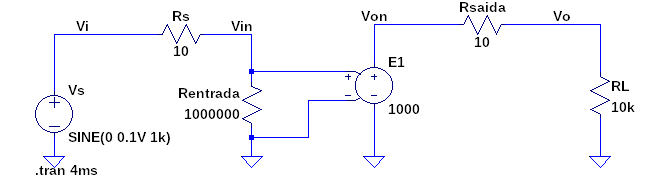
\includegraphics[scale=0.5]{ltspicetras.png}
\caption{Circuito modelado no ltspice fonte senoidal}
\label{Rotulo}
\end{figure}
Realizou-se duas simulações a primeira manteve-se a fonte de tensão controlada por tensão, também mostrada na figura 3. O resultado da simulação para o ganho esta mostrado na figura 4
\begin{figure}[H]
\centering
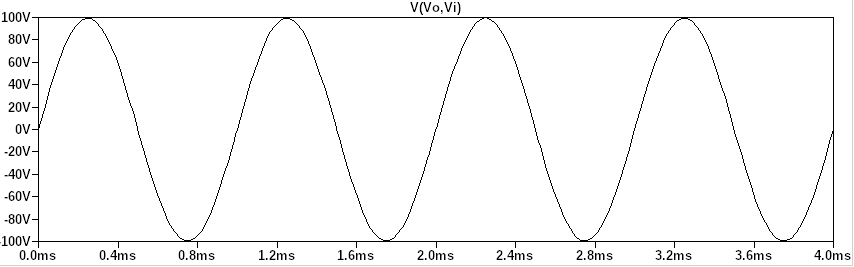
\includegraphics[scale=0.5]{grafico.png}
\caption{Circuito modelado no ltspice fonte senoidal}
\label{Rotulo}
\end{figure}

Para a segunda simulação o modelo do amplificador será  arbitrary behavioral voltage source, com tensão limitada  +5V e em -5V, mostrada na figura 5

\begin{figure}[H]
\centering
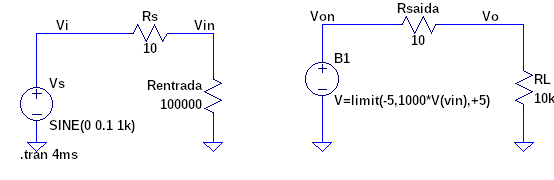
\includegraphics[scale=0.5]{ltspicelimit.png}
\caption{Circuito modelado no arbitrary behavioral voltage source limitada}
\label{Rotulo}
\end{figure}

Utilizando ainda os valores da última linha da tabela anterior podemos perceber um corte abrupto mostrado na figura 6

\begin{figure}[H]
\centering
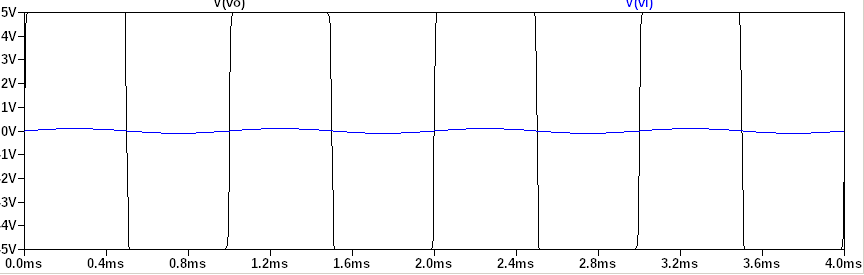
\includegraphics[scale=0.5]{corte.png}
\caption{Simulação tensão de saturação}
\label{Rotulo}
\end{figure}

\subsection{Resultados}
Pode-se observar na primeira simulação utilizando uma fonte controlada por tensão, não teve um corte na simulação devido não ter um limite para tensão $V_{sensor}$,  já no segundo caso pode-se observar que ocorreu um corte em 5V ou seja a tensão de entrada $V_{sensor}$, mostrado na figura 6 
\end{document}
